\chapter{Estado del arte del perfilado de autor}
\label{chap:estadoarte}

Durante los inicios del perfilado automático de autor, los algoritmos se centraban en la tarea de la clasificación por género.
En esta línea, trabajos como Koppel et al., 2002 \cite{koppel2002automatically} se desmarcaban de la tendencia de la época,
la cual se basaba en la clasificación de textos en base a su contenido, para enfocarse en la clasificación de textos en base a su estilo.
En este caso, se centraban en la obtención del género del autor mediante el análisis
de 920 documentos de carácter formal escritos en inglés con una media de alrededor de 34.300 palabras cada uno, obteniendo una precisión en la clasificación de
aproximadamente el 77\%.

\bigskip
Así, la demostración de la existencia de rasgos diferenciadores en la escritura que permitían perfilar ciertos ascpectos del individuo, especialmente del género, 
supuso un gran avance en el campo del perfilado de autor
y dió pié a la realización de trabajos como (Argamon et al., 2003) \cite{argamon2003gender}, (Corney et.al, 2002) \cite{corney2002gender} o (Otterbacher et al., 2010) \cite{otterbacher2010inferring}, 
así como también permitió el inicio de una clasificación más compleja en base a otras características demográficas.

\bigskip
Posteriormente, en los años siguientes, tal como recoge Wiegmann et al., 2019 \cite{wiegmann2019overview}, se continuarían llevando a cabo estudios en esta línea, diversificando
las características a clasificar. En este sentido, se realizarían trabajos como Álvarez-Carmona et al., 2018 \cite{alvarez2018overview}, donde se buscaba
predecir el lugar de residencia del autor junto a su ocupación; otros como Volkova et al., 2015 \cite{volkova2015predicting}, en el que se trataba de perfilar la orientación política,
el salario, el optimismo del autor o su sentimiento de satisfacción vital; Preoţiuc-Pietro et al., 2018 \cite{preoctiuc2018user}, en el que se llevaba a cabo la tarea de
clasificar la raza y la etnia del autor; u otros como Fatima et al., 2017 \cite{fatima2017multilingual} que buscaban extender el perfilado de autor a otros idiomas. Asimismo,
la mayor parte de los \textit{datasets} utilizados para la creación de los modelos con estos algoritmos, se basaban en textos de redes sociales como Twitter (Burger et al., 2011) \cite{burger2011discriminating},
Facebook (Fatima et al., 2017) \cite{fatima2017multilingual} o Reddit (Gjurković et al., 2018) \cite{gjurkovic2018reddit}, reflejando así la importancia de estas plataformas
en la actualidad.

\bigskip
Por otro lado, en el año 2011, se celebraría el primer evento organizado por el \textit{PAN} (\textit{Plagiarism Analysis, Authorship Identification, and Near-Duplicate Detection}) \cite{pan},
uno de los foro de investigación más importantes que organiza eventos científicos y tareas anuales relacionadas con el análisis forense de textos digitales
y rasgos estilométricos, así como uno de los grandes implusores del perfilado de autor. La primera de las tareas centrada en este campo se celebraría en el año 2013 (Rangel et al., 2013) \cite{rangel2013overview},
en la que se pedía a los participantes que obtuvieran, a partir de una serie de \textit{tweets}, la edad y el género de su autor. El ganador de este concurso obtuvo una
precisión del 60\% en la clasificación de género y del 67\% en la clasificación de edad, haciendo uso, la mayor parte de los participantes, de técnicas de aprendizaje
supervisado como los Árboles de Decisión (en inglés \textit{Decission Trees}) o las Máquinas de Soporte Vectorial (en inglés \textit{Support Vector Machines}) e inluyendo
en sus modelos características basadas en el TF-IDF, n-gramas, etiquetas POS u otras como el número de emoticonos o la frecuencia de signos de puntuación.
En los siguientes años se celebrarían nuevas ediciones con el perfilado de autor en el centro (Rangel et al., 2014 \cite{rangel2014overview}; Rangel et al., 2015 \cite{rangel2015overview};
Rangel et al., 2016 \cite{rangel2016overview}...), en las que se añadiríán nuevas sub-tareas como el reconocimiento de rasgos personales, la ocupación o los dialectos del lenguaje,
así como también alcanzando mejores resultados en la clasificación.

\section{Conceptos básicos}

Cuando hablamos del perfilado automático de autores, nos referimos a la tarea del análisis detallado de un texto para la obtención de ciertas características
que nos permitan identificar a su autor.
Dicha tarea de análisis está enmarcada dentro del campo del Procesado del Lenguaje Natural (\textit{Natural Language Processing} o NLP en inglés) y, más concretamente,
dentro de la rama de la Estilometría. De esta forma, para las tareas de NLP se hace uso
de una serie de algoritmos y técnicas básicas que permiten la extracción de características numéricas y objetivas de un texto. Las más utilizadas y relevantes
para la comprensión de este trabajo son las siguientes:

\subsection{TF-IDF}
El TF-IDF (del inglés \textit{Term Frequency-Inverse Document Frequency}) es una medida numérica muy utilizada en el campo de la recuperación de información 
(en inglés \textit{Information Retrieval} o IR) que expresa cuán relevante es una palabra para un documento en una colección.

\bigskip
El cálculo de dicha medida para cada palabra sigue la siguiente fórmula:

\begin{equation}
		\label{eq:tfidf}
		\text{TF-IDF}(t,d) = \text{TF}(t,d) \times \text{IDF}(t)
\end{equation}

Donde:
\begin{itemize}
	\item $t$ es la palabra de la que se quiere calcular el TF-IDF.
	\item $d$ es el documento en el que se encuentra la palabra.
	\item $\text{TF}(t,d)$ es la frecuencia de la palabra $t$ en el documento $d$, que se calcula como:
		\begin{equation}
				\label{eq:tf}
				TF(t,d) = \frac{n_{t,d}}{n_d}
		\end{equation}

		Donde:
		\begin{itemize}
				\item $n_{t,d}$ es el número de veces que la palabra $t$ aparece en el documento $d$.
				\item $n_d$ es el número total de palabras en el documento $d$.
		\end{itemize}

	\item $\text{IDF}(t)$ es la frecuencia inversa de documentos que representa la importancia de la palabra $t$ en la colección de documentos y
		se calcula como:
		\begin{equation}
			\label{eq:idf}
			\text{IDF}(t) = \log \left(\frac{N}{\text{DF}(t)}\right)
		\end{equation}

		Donde:
		\begin{itemize}
				\item $N$ es el número total de documentos en la colección.
				\item $\text{DF}(t)$ es el número de documentos en los que aparece la palabra $t$.
		\end{itemize}
\end{itemize}

\bigskip
Por lo tanto, la importancia aumenta proporcionalmente al número de veces que una palabra aparece en el documento, pero se compensa con la frecuencia 
de la palabra en la colección, lo que permite manejar el hecho de que algunas palabras son generalmente más comunes que otras.

\subsection{Etiquetas POS}

Las etiquetas POS (\textit{Part-Of-Speech} en inglés) son etiquetas gramaticales que se asignan a las palabras de un texto según su función sintáctica, es
decir, si se trata de un sustantivo, un verbo, un adjetivo, etc.
Existen varios tipos de etiquetas POS, pero las más empleadas son las descritas en el \textit{Penn Treebank Project} \cite{marcus1993building}.

\subsection{N-gramas}

Los n-gramas son una técnica de modelado de lenguaje que consiste en la extracción de secuencias de $n$ elementos de un texto. Existen n-gramas de varios tipos
en los que se pueden extraer secuencias de caracteres, palabras, etiquetas POS, etc. Los más habituales son los bigramas y los trigramas (\textit{bigrams} y \textit{trigrams} en inglés).

\subsection{\textit{Bag-of-words}}

La \textit{bag-of-words} o BoW es una técnica simple de representación de documentos que consiste en la extracción de las palabras que aparecen en un texto,
sin tener en cuenta el orden en el que aparecen ni la estructura gramatical de la que forman parte. De esta modo, se obtiene un vector de características en el 
que cada posición representa una palabra y que tiene como valores el número de veces que aparece dicha palabra en el documento.

\subsection{Análisis Semántico Latente}
\label{sec:analisis_semantico_latente}

El Análisis Semántico Latente (\textit{Latent Semantic Analysis} o LSA en inglés) es una técnica de IR desarrollada por Deerwester et al., 1990 \cite{deerwester1990indexing}
que busca descubrir relaciones latentes
entre las palabras y los documentos que forman una colección. Esta técnica se basa
en el idea de que las palabras que aparecen en contextos similares
tienden a tener significados similares. Para aplicarla, se construye una matriz en la que se almacena la frecuencia de cada palabra del vocabulario en cada documento y
a continuación, se aplica una descomposición en valores singulares (\textit{Singular Value Decomposition} o SVD en inglés) a dicha matriz para reducir su dimensionalidad
y encontrar relaciones palabras-documentos.

\bigskip
Esta técnica tiene limitaciones, sobre todo a la hora de manejar sinónimos y polisemias ya que, al basarse únicamente en patrones estadísticos,
no tiene en cuenta el significado real de las palabras.

\section{Competiciones analizadas}
\label{sec:competiciones_analizados}

Una vez explicados los conceptos básicos, procederemos en esta sección al análisis de las competiciones más relevantes en el contexto
del perfilado automático de autores. En este sentido, destacar que, ya que el objetivo de este trabajo estaba encuadrado en
la investigación sobre algoritmos de perfilado de autores de habla inglesa, se obviaron otras competiciones relevantes como pueden ser
las organizadas por IberLEF \cite{iberlef}, un foro de investigación que promueve el desarrollo de sistemas basados en NLP en español y otras
lenguas ibéricas.
Asimismo, dado que el perfilado de la edad era otra característica fundamental que debía incluir este trabajo, se seleccionaron aquellas competiciones
que contaban con dicha tarea, en este caso, las celebradas en los años 2014 (Rangel et al.) \cite{rangel2014overview}, 2015 (Rangel et al.) \cite{rangel2015overview} y 2019 (Wiegmann et al.) \cite{wiegmann2019overview}.

\subsection{\textit{PAN Author Profiling 2014}}

Esta segunda edición de la competición internacional de perfilado de autores celebrada en 2014 por PAN, estaba enfocada en la clasificación de género y edad de los autores, en la que se consideraban, para esta última, las siguientes
clases: 18-24, 25-34, 35-49, 50-64, 65-XX.

\subsubsection{\textit{Corpus}}

En lo referente al \textit{dataset} de entrenamiento y evaluación utilizado, la organización de la
competición elaboró un \textit{corpus} con documentos de diferentes tipos que incluían: \textit{tweets}, \textit{posts} de blogs, \textit{posts} de otras redes sociales y \textit{reviews} de hoteles.
Todos ellos contenían documentos en inglés y en español a excepción de las \textit{reviews} de hoteles, las cuales solo estaban disponibles en inglés.

\bigskip
Como se puede observar en la distribución de los autores, disponible tanto en la Tabla \ref{tab:dataset_2014} como en la Figura \ref{fig:dataset_2014}, el número de autores de habla inglesa
es muy superior a los de habla española, lo que provoca potencialmente que los algoritmos entrenados con este \textit{dataset} tengan una mejor generalización y obtengan, por lo tanto,
mejores predicciones para la lengua inglesa. Asimismo, existe un amplio desbalanceo de clases con respecto a la edad en el \textit{corpus},
donde las clases 18-24 y 65-XX cuentan con un número de autores significativamente inferior al resto de clases. Destacar finalemente que,
en cuanto al género, el \textit{dataset} está perfectamente balanceado, existiendo el mismo número de autores masculinos y femeninos, lo que
ayuda a evitar un posible sesgo.

\bigskip
\begin{figure}[H]
	\centering
	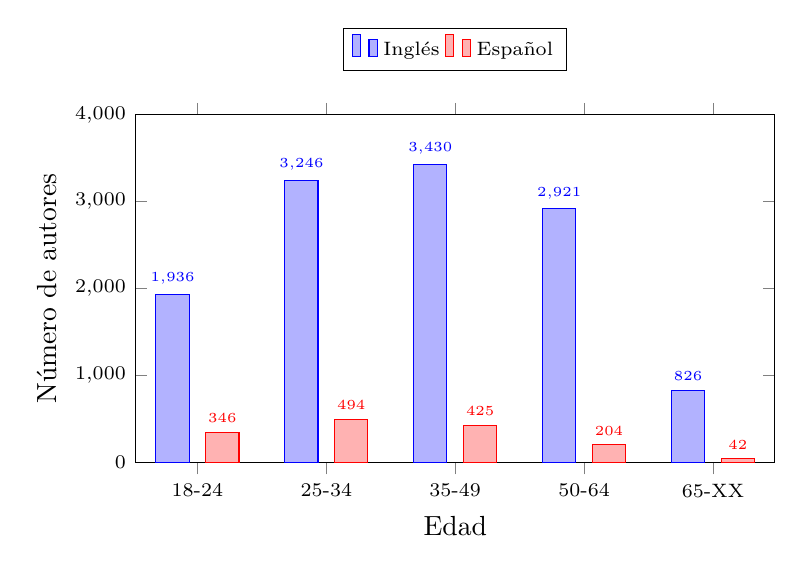
\begin{tikzpicture}
			\begin{axis}[
					width=0.8\textwidth,
					height=6cm,
					xmajorgrids=false,
					x tick label style={/pgf/number format/1000 sep=},
					x tick label style={font=\scriptsize},
					y tick label style={font=\scriptsize},
					ylabel=Número de autores,
					xlabel=Edad,
					ybar=6pt,
					bar width=12pt,
					enlarge x limits=0.12,
					nodes near coords,
					nodes near coords style={font=\tiny},
					symbolic x coords={18-24, 25-34, 35-49, 50-64, 65-XX},
					xtick=data,
					ymin=0,
					ymax=4000,
					legend style={at={(0.5,1.25)},font=\scriptsize, anchor=north,legend columns=-1},
			]
			\addplot table[x=Edad,y=Inglés] {
					Edad    Inglés
					18-24   1936
					25-34   3246
					35-49   3430
					50-64   2921
					65-XX   826
			};
			\addplot table[x=Edad,y=Español] {
					Edad    Español
					18-24   346
					25-34   494
					35-49   425
					50-64   204
					65-XX   42
			};
			\legend{Inglés, Español}
			\end{axis}
	\end{tikzpicture}
	\caption{Comparativa del número de autores por idioma en el \textit{corpus} del \textit{PAN Author Profiling 2014}}
	\label{fig:dataset_2014}
\end{figure}

\bigskip
\begin{table}[H]
	\centering
	\resizebox{0.7\textwidth}{!}{
		\rowcolors{2}{white}{udcgray!25}
		\begin{tabular}{|c|c|c|c|c|}
			\hhline{~|----|}
			\multicolumn{1}{c|}{\cellcolor{white}} & \multicolumn{2}{c|}{\cellcolor{udcpink!25}\textbf{Entrenamiento}} & \multicolumn{2}{c|}{\cellcolor{udcpink!25}\textbf{Test}} \\ \hline
			\textbf{Edad} & \textbf{Inglés} & \textbf{Español} & \textbf{Inglés} & \textbf{Español} \\ \hline
			18-24 & 1,936 & 346 & 850 & 158  \\ \hline
			25-34 & 3,246 & 494 & 1,380 & 218  \\ \hline
			35-49 & 3,430 & 425 & 1,470  & 210 \\ \hline
			50-64 & 2,921 & 204 & 1,226 & 92 \\ \hline
			65-XX & 826 & 42 & 324 & 32 \\ \hline
			\textbf{Total} & \textbf{12,359} & \textbf{1,511} & \textbf{5,250} & \textbf{710} \\ \hline
		\end{tabular}
	}
	\caption{Distribución del número de autores en cada rango de edad en el \textit{corpus} del \textit{PAN Author Profiling 2014}}
	\label{tab:dataset_2014}
\end{table}

\subsubsection{\textit{Resultados}}

Basándonos en los resultados de la competición, reflejados en la Tabla \ref{tab:algoritmos_2014}, podemos observar que los mejores datos de precisión
en cuanto a género fueron de alrededor de un 60\% para ambos idiomas, mientras que para la edad fueron de aproximadamente un 40\% para el inglés y de
un 50\% para el español.

\bigskip
En cuanto a las aproximaciones algorítmicas llevadas a cabo por los equipos mejor clasificados en la competición, podemos destacar lo siguiente:

\begin{itemize}
	\item \textbf{Preprocesado}: En cuanto al preprocesado, tanto Maharjan et al. \cite{maharjan2014simple} como Weren et al. \cite{weren2014exploring} realizaron un limpiado de los documentos XML para obtener
	texto plano, escapando caracteres inválidos en el caso del segundo equipo.
	\item \textbf{\textit{Features}}: En relación a las características extraídas de los documentos para la clasificación, Maharjan \cite{maharjan2014simple}, Weren et al. \cite{weren2014exploring} y Siang et al.,
	consideraron diferentes rasgos estilométricos como la frecuencia de los signos de puntuación, el tamaño de las frases o la frecuencia de las palabras, entre otros. Con respecto 
	a los rasgos basados en el contenido, Siang et al. y Maharjan et al. \cite{maharjan2014simple}, modelizaron el lenguaje con \textit{bag-of-word} y n-gramas, respectivamente, mientras
	que López-Monroy et al. \cite{lopez2014using} emplearon representaciones más complejas basadas en las relaciones entre palabras y documentos, explicadas a fondo
	en su trabajo.
	\item \textbf{Clasificación}: En cuanto a los algoritmos de clasificación utilizados, todos los equipos que aparecen en la Tabla \ref{tab:algoritmos_2014} emplearon regresión logística. López-Monroy et al. \cite{lopez2014using}
	hizo uso, más concretamente, de una librería de regresión logística y de SVMs lineales llamada LIBLINEAR (\textit{Large Linear Classification}) \cite{fan2008liblinear}.
\end{itemize}

\bigskip
\begin{table}[H]
	\centering
	\resizebox{0.9\textwidth}{!}{
		\rowcolors{2}{white}{udcgray!25}
		\setlength{\tabcolsep}{7pt}
		\begin{tabular}{|c|c|c|c|c|c|c|c|}
			\hhline{~|-------|}
			\multicolumn{1}{c|}{\cellcolor{white}} & \multicolumn{7}{c|}{\cellcolor{udcpink!25}\textbf{Precisión}} \\
			\hhline{~|-------|}
			\multicolumn{1}{c|}{\cellcolor{white}} & \multicolumn{3}{c|}{\textbf{Global}}  & \multicolumn{2}{c|}{\textbf{Inglés}} & \multicolumn{2}{c|}{\textbf{Español}} \\ \hline
			\textbf{Equipo participante} & \textbf{Conjunta} & \textbf{Género} & \textbf{Edad} & \textbf{Género} & \textbf{Edad} & \textbf{Género} & \textbf{Edad} \\ \hline
			López-Monroy et al. 2014 \cite{lopez2014using} & 0.2790 & 0.6310 & 0.4421 & 0.6512  & 0.3950 & 0.6108 & 0.4892 \\ \hline
			Siang et al. & 0.2758 & 0.6344 & 0.4348 & 0.663 & 0.3909 & 0.6057 & 0.4786 \\ \hline
			Maharjan et al., 2014 \cite{maharjan2014simple} & 0.2624 & 0.5948 & 0.4411 & 0.6132 & 0.3811 & 0.5764 & 0.5010 \\ \hline
			Weren et al., 2014 \cite{weren2014exploring} & 0.2266 & 0.5866 & 0.3863 & 0.6066 & 0.3690 & 0.5666 & 0.4035 \\ \hline
		\end{tabular}
	}
	\caption{Cuatro mejores clasificados en la competición \textit{PAN Author Profiling 2014}}
	\label{tab:algoritmos_2014}
\end{table}

\subsection{\textit{PAN Author Profiling 2015}}

En esta competición, a mayores de la clasificación por género y edad del autor, se añadió la predicción de rasgos de la personalidad. En concreto,
se buscaba predecir los cinco rasgos descritos en el modelo \textit{Big Five} (Goldberg, 1990) \cite{goldberg1990alternative}: extroversión (\textit{extroversion}),
estabilidad emocional / neuroticismo (\textit{stability / neuroticism}), apertura a la experiencia (\textit{openness to experience}), amabilidad (\textit{agreeableness}) y
responsabilidad (\textit{conscientiousness}). En cuanto a la edad, y a diferencia de la edición anterior de 2014, se eliminó la categoría de 65 años o más,
resultando en cuatro categorías: 18-24, 25-34, 35-49 y 50-XX.

\subsubsection{\textit{Corpus}}

\bigskip
En lo que respecta al \textit{corpus} proporcionado para la competición, los organizadores recopilaron \textit{tweets} de la red social Twitter
de 726 usuarios en cuatro idiomas diferentes: inglés, español, italiano y holandés. Dicho \textit{dataset} está etiquetado con el género y la edad
(solamente para inglés y español) de los autores, que ellos mismos reportaron en sus perfiles de Twitter. Para determinar los rasgos de la personalidad,
los autores completaron el test BFI-10 (Rammstedt et al., 2007) \cite{rammstedt2007measuring}, proporcionando valores para cada rasgo normalizados entre -0.5 y 0.5.

\bigskip
Así, como se puede ver en la Figura \ref{fig:dataset_2015}, el \textit{dataset} vuelve a estar desbalanceado en cuanto a la edad, ya que existen
clases como la 50-XX la cual apenas tiene un 7\% de la representación con respecto al total. Sin embargo,
a excepción de la clase 18-24, existe un número similar de autores de habla española e inglesa, por lo que cabe esperar una generalización
similar para ambos idiomas. En lo referente a la ditribución de género, como se puede ver en la Tabla \ref{tab:dataset_2015}, está perfectamente balanceada,
contando con un 50\% de autores de cada género para todos los idiomas.

\bigskip
\begin{figure}[H]
	\centering
	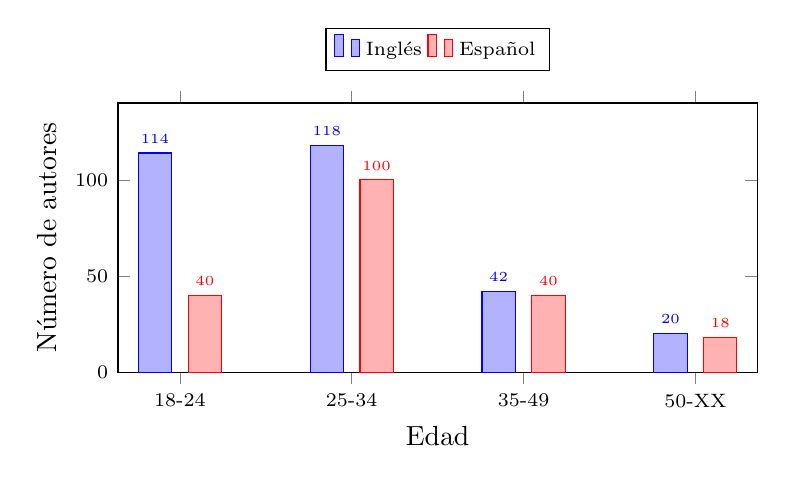
\begin{tikzpicture}
			\begin{axis}[
					width=0.8\textwidth,
					height=5cm,
					xmajorgrids=false,
					x tick label style={/pgf/number format/1000 sep=},
					x tick label style={font=\scriptsize},
					y tick label style={font=\scriptsize},
					ylabel=Número de autores,
					xlabel=Edad,
					ybar=6pt,
					bar width=12pt,
					enlarge x limits=0.12,
					nodes near coords,
					nodes near coords style={font=\tiny},
					symbolic x coords={18-24, 25-34, 35-49, 50-XX},
					xtick=data,
					ymin=0,
					ymax=140,
					legend style={at={(0.5,1.28)},font=\scriptsize, anchor=north,legend columns=-1},
			]
			\addplot table[x=Edad,y=Inglés] {
					Edad    Inglés
					18-24   114
					25-34   118
					35-49   42
					50-XX   20
			};
			\addplot table[x=Edad,y=Español] {
					Edad    Español
					18-24   40
					25-34   100
					35-49   40
					50-XX   18
			};
			\legend{Inglés, Español}
			\end{axis}
	\end{tikzpicture}
	\caption{Comparativa del número de autores por idioma en el \textit{corpus} del \textit{PAN Author Profiling 2015}}
	\label{fig:dataset_2015}
\end{figure}

\bigskip
\begin{table}[H]
	\centering
	\resizebox{0.9\textwidth}{!}{
		\rowcolors{2}{white}{udcgray!25}
		\setlength{\tabcolsep}{8pt}
		\begin{tabular}{|c|c|c|c|c|c|c|c|c|}
			\hhline{~|--------|}
			\multicolumn{1}{c|}{\cellcolor{white}} & \multicolumn{4}{c|}{\cellcolor{udcpink!25}\textbf{Entrenamiento}} & \multicolumn{4}{c|}{\cellcolor{udcpink!25}\textbf{Test}} \\ \hline
			\textbf{Característica} & \textbf{Inglés} & \textbf{Español} & \textbf{Italiano} & \textbf{Holandés} & \textbf{Inglés} & \textbf{Español} & \textbf{Italiano} & \textbf{Holandés} \\ \hline
			18-24 & 58 & 22 & - & - & 56 & 18 & - & -  \\ \hline
			25-34 & 60 & 56 & - & - & 58 & 44 & - & - \\ \hline
			35-49 & 22 & 22 & - & - & 20  & 18 & - & - \\ \hline
			50-XX & 12 & 10 & - & - & 8 & 8 & - & - \\ \hline
			\hline
			Masculino & 76 & 55 & 19 & 17 & 71 & 44 & 18 & 16 \\ \hline
			Femenino & 76 & 55 & 19 & 17 & 71 & 44 & 18 & 16 \\ \hline
			\hline
			Extrovertido & 0.16 & 0.18 & 0.17 & 0.24 & 0.17 & 0.16 & 0.15 & 0.24 \\ \hline
			Estabilidad & 0.14 & 0.07 & 0.20 & 0.21 & 0.13 & 0.09 & 0.20 & 0.22 \\ \hline
			Amabilidad & 0.12 & 0.14 & 0.22 & 0.13 & 0.14 & 0.14 & 0.19 & 0.15 \\ \hline
			Responsabilidad & 0.17  & 0.24 & 0.18 & 0.14 & 0.17 & 0.21 & 0.21 & 0.17 \\ \hline
			Apertura & 0.24 & 0.18 & 0.23 & 0.29 & 0.26 & 0.19 & 0.25 & 0.28 \\ \hline
		\end{tabular}
	}
	\caption{Distribución de los autores por característica y lenguaje en el \textit{corpus} del \textit{PAN Author Profiling 2015}}
	\label{tab:dataset_2015}
\end{table}

\subsubsection{\textit{Resultados}}

A la vista de los datos de precisión obtenidos por los primeros equipos clasificados, mostrados en la Tabla \ref{tab:algoritmos_2015},
podemos determinar que existe una gran mejora con respecto a los resultados de la competición anterior del año 2014, mejorando
la clasificación conjunta de edad y género en aproximadamente un 40\%.

\bigskip
Más en concreto, destacar los grandes resultados que
ofrecen los algoritmos presentados con respecto al género en los dos idiomas principales del \textit{corpus}, llegando a alcanzar
precisiones del 96\% para el español en el caso de Alvarez-Carmona et al. \cite{alvarez2015inaoe}. Con respecto a la edad,
se puede ver como se obtienen unos mejores resultados, de alrededor de un 5\%, en la clasificación en inglés que en español, algo que
hipotéticamente puede ser un reflejo de las pequeñas diferencias existentes entre el número de autores en cada uno de los idiomas en
el \textit{dataset} de entrenamiento.

\bigskip
Con respecto a la implementación de los algoritmos, podemos destacar lo siguiente:

\begin{itemize}
	\item \textbf{Preprocesado}: De forma similar a los algoritmos de años anteriores, la mayoría realizaron una limpieza del HTML incluído
	en los \textit{tweets} y, tanto González-Gallardo et al. \cite{gonzalez2015tweets} como Grivas et al. \cite{grivas2015author}, utilizaron
	las menciones, los \textit{hashtags} y los enlaces como características adicionales.
	\item \textbf{\textit{Features}}: En la mayor parte de los algoritmos presentados, se combinaba el uso de características
	basadas en el estilo y en el contenido. Así, en cuanto a contenido, González-Gallardo et al. \cite{gonzalez2015tweets} hizo uso de n-gramas de caracteres
	mientras que Grivas et al. \cite{grivas2015author} empleó n-gramas basados en TF-IDF. Además, en el caso de Grivas et al. \cite{grivas2015author},
	se analizaron otras caracterísitcas basadas en el estilo como la longitud de las palabras o el número de mayúsculas. En el caso de Alvarez-Carmona et al. \cite{alvarez2015inaoe},
	se hizo uso del Análisis Semántico Latente, explicado en la Sección \ref{sec:analisis_semantico_latente}, junto a una técnica similar a la empleada por
	López-Monroy et al. \cite{lopez2014using} en el año 2014.
	\item \textbf{Clasificación}: En lo referente a los métodos utilizados para realizar las predicciones, destaca el uso de la librería LIBLINEAR \cite{fan2008liblinear}
	por parte de Alvarez-Carmona et al. \cite{alvarez2015inaoe} y González-Gallardo et al. \cite{gonzalez2015tweets}. En el caso de Grivas et al. \cite{grivas2015author}, se hizo
	uso de SVMs para la clasificación del género y la edad mientras que se emplearon SVRs (Drucker et al., 1996) \cite{drucker1996support} para el reconocimiento de los rasgos personales.
\end{itemize}

\begin{table}[H]
	\centering
	\resizebox{\textwidth}{!}{
		\rowcolors{2}{white}{udcgray!25}
		\setlength{\tabcolsep}{6pt}
		\begin{tabular}{|c|c|c|c|c|c|c|c|c|c|}
			\hhline{~|---------|}
			\multicolumn{1}{c|}{\cellcolor{white}} & \multicolumn{9}{c|}{\cellcolor{udcpink!25}\textbf{Precisión}} \\
			\hhline{~|---------|}
			\multicolumn{1}{c|}{\cellcolor{white}} & \multicolumn{3}{c|}{\textbf{Global}} & \multicolumn{2}{c|}{\textbf{Inglés}} & \multicolumn{2}{c|}{\textbf{Español}} & \multicolumn{1}{c|}{\textbf{Italiano}} & \multicolumn{1}{c|}{\textbf{Holandés}} \\ \hline
			\textbf{Equipo participante} & \textbf{Conjunta} & \textbf{Género} & \textbf{Edad} & \textbf{Género} & \textbf{Edad} & \textbf{Género} & \textbf{Edad} & \textbf{Género} & \textbf{Género} \\ \hline
			Alvarez-Carmona et al. 2015 \cite{alvarez2015inaoe} & 0.7116 & 0.8712 & 0.8168 & 0.8592 & 0.8380 & 0.9659 & 0.7955 & 0.7222 & 0.9375 \\ \hline
			González-Gallardo et al., 2015 \cite{gonzalez2015tweets} & 0.6693 & 0.8871 & 0.7545 & 0.8521 & 0.7817 & 0.8977 & 0.7273 & 0.8611 & 0.9375 \\ \hline
			Grivas et al., 2015 \cite{grivas2015author} & 0.6487 & 0.9011 & 0.7199 & 0.8592 & 0.7465 & 0.9432 & 0.6932 & 0.8333 & 0.9688 \\ \hline
			Kocher et al., 2015 \cite{kocher2015unine} & 0.5655 & 0.7800 & 0.7250 & 0.7113 & 0.7113 & 0.8182 & 0.7386 & 0.7778 & 0.8125 \\ \hline
		\end{tabular}
	}
	\caption{Cuatro mejores clasificados en la competición \textit{PAN Author Profiling 2015}}
	\label{tab:algoritmos_2015}
\end{table}

\subsection{\textit{PAN Celebrity Profiling 2019}}

En esta última competición, la primera de ellas celebrada específicamente para el perfilado de celebridades, la tarea consistía en predecir
cuatro caracterísitcas demográficas a partir de sus publicaciones en Twitter:

\begin{itemize}
	\item \textbf{Género}: Masculino, femenino o no binario.
	\item \textbf{Año de nacimiento}: A la hora de calcular la precisión del algoritmos,
		se contemplará una ventana de error adaptativa entre los 2 y los 9 años en función de la edad real de la celebridad. 
	\item \textbf{Ocupación o motivo de fama}: Deportista (\textit{sports}), actor (\textit{performer}), político (\textit{politics}), creador de contenido (\textit{creator}),
		director (\textit{manager}), científico (\textit{science}), professional (\textit{professional}) o religioso (\textit{religious}).
	\item \textbf{Fama}: Revelación (\textit{rising}), estrella (\textit{star}) o superestrella (\textit{superstar}).
\end{itemize}

\subsubsection{\textit{Corpus}}

En este caso, como se mencionó anteriormente, el \textit{corpus} empleado está compuesto por publicaciones en inglés en la red social Twitter. En concreto,
el \textit{dataset} contenía un total de 48.335 celebridades con aproximadamente 2.180 \textit{tweets} cada una. El \textit{corpus} fue obtenido
a partir del \textit{Webis Celebrity Profiling Corpus} (Wiegmann et al., 2019) \cite{wiegmann2019celebrity}, en el cual se relacionaban los perfiles
de Twitter de las celebridades con sus entradas en Wikidata. De esta forma, se obtuvieron los \textit{tweets} de sus \textit{timelines} de la red social
y se simplificaron las caracterísitcas demográficas que ofrecía Wikidata, filtrando finalmente las celebridades nacidas antes de 1940 y que no tuvieran
el inglés como lengua de uso principal.

\bigskip
\begin{figure}[H]
	\centering
	\begin{subfigure}{0.5\textwidth}
			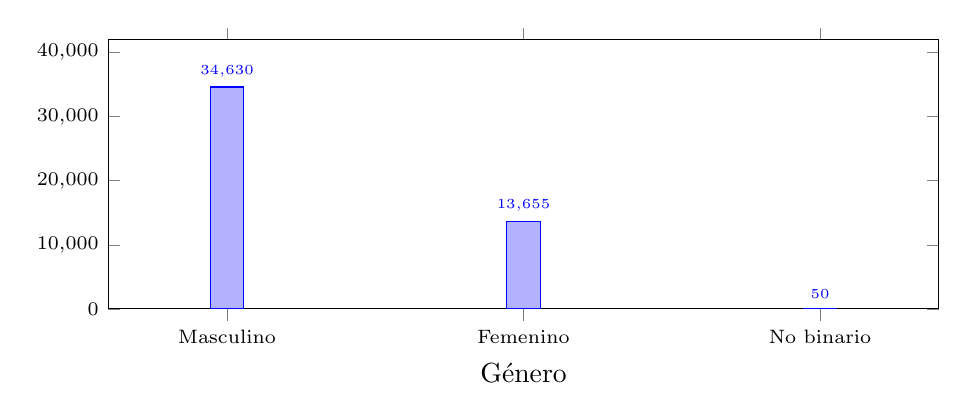
\begin{tikzpicture}
					\begin{axis}[
							width=\linewidth,
							height=5cm,
							xmajorgrids=false,
							x tick label style={font=\scriptsize},
							y tick label style={font=\scriptsize},
							ybar=6pt,
							bar width=12pt,
							enlarge x limits=0.2,
							ymin=0,
							ymax=42000,
							nodes near coords,
							nodes near coords style={font=\tiny},
							xtick=data,
							xticklabels={Masculino, Femenino, {No binario}},
							xlabel={Género},
							scaled y ticks=false
					]
					\addplot coordinates {(1,34630) (2,13655) (3,50)};
					\end{axis}
			\end{tikzpicture}
			\label{fig:distribucion_genero_2019}
	\end{subfigure}%
	\hfill
	\begin{subfigure}{0.5\textwidth}
			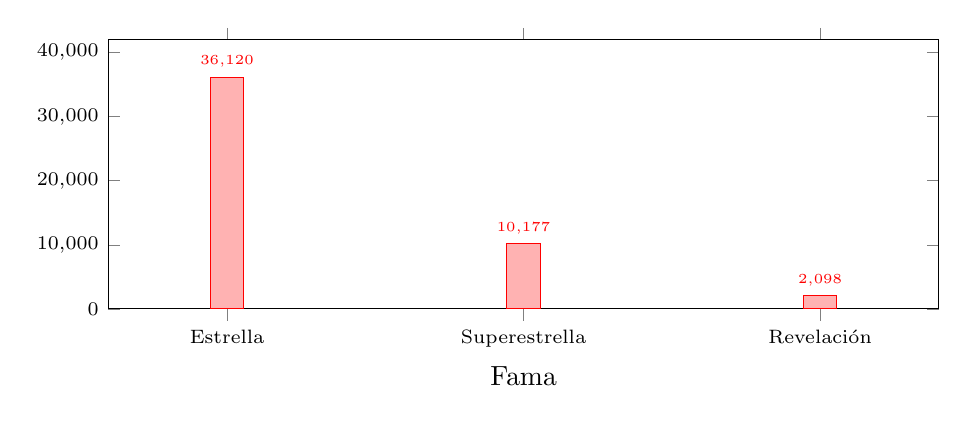
\begin{tikzpicture}
					\begin{axis}[
							width=\linewidth,
							height=5cm,
							xmajorgrids=false,
							x tick label style={font=\scriptsize},
							y tick label style={font=\scriptsize},
							ybar=6pt,
							bar width=12pt,
							enlarge x limits=0.2,
							ymin=0,
							ymax=42000,
							nodes near coords,
							nodes near coords style={font=\tiny},
							xtick=data,
							xticklabels={Estrella, Superestrella, Revelación},
							xlabel={Fama},
							scaled y ticks=false
					]
					\addplot[color=red, fill=red!30] coordinates {(1,36120) (2,10177) (3,2098)};
					\end{axis}
			\end{tikzpicture}
			\label{fig:distribucion_fama_2019}
	\end{subfigure}
	\caption{Distribuciones de género y fama en el \textit{corpus} de la competición \textit{PAN Celebrity Profiling 2019}.}
	\label{fig:distribuciones_2019}
\end{figure}

\begin{figure}[H]
	\centering
	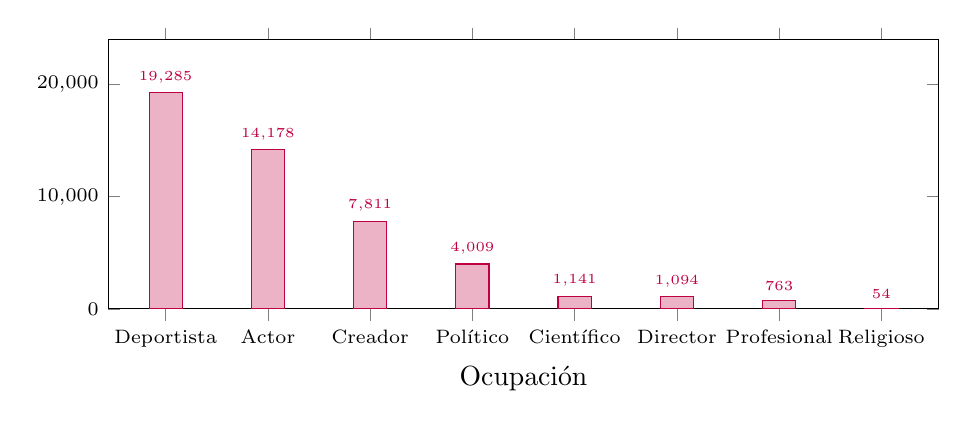
\begin{tikzpicture}
		\begin{axis}[
				width=\linewidth,
				height=5cm,
				xmajorgrids=false,
				x tick label style={font=\scriptsize},
				y tick label style={font=\scriptsize},
				ybar=6pt,
				bar width=12pt,
				enlarge x limits=0.08,
				ymin=0,
				ymax=24000,
				nodes near coords,
				nodes near coords style={font=\tiny},
				xtick=data,
				xticklabels={Deportista, Actor, Creador, Político, Científico, Director, Profesional, Religioso},
				xlabel={Ocupación},
				scaled y ticks=false
		]
		\addplot[color=purple, fill=purple!30] coordinates {(1,19285) (2,14178) (3,7811) (4,4009) (5,1141) (6,1094) (7,763) (8,54)};
		\end{axis}
	\end{tikzpicture}
	\label{fig:distribucion_ocupacion_2019}
	\caption{Distribución de ocupaciones en el \textit{corpus} de la competición \textit{PAN Celebrity Profiling 2019}.}
\end{figure}

\begin{table}[H]
	\centering
	\resizebox{0.8\textwidth}{!}{
		\rowcolors{2}{white}{udcgray!25}
		\begin{tabular}{|c|c|c|c|}
			\hhline{~|---|}
			\multicolumn{1}{c|}{\cellcolor{white}} & \multicolumn{3}{c|}{\cellcolor{udcpink!25}\textbf{Precisión}} \\ \hline
			\textbf{Equipo participante} & \textbf{Conjunta} & \textbf{Género} & \textbf{Edad} \\ \hline
			Radivchev et al. 2019 \cite{radivchev2019celebrity} & 0.477 & 0.928 & 0.514  \\ \hline
			Martinc et al., 2019 \cite{martinc2019hot} & 0.410 & 0.906 & 0.453 \\ \hline
			Fernquist et al., 2019 & 0.362 & 0.774 & 0.468 \\ \hline
			Moreno-Sandoval et al., 2019 \cite{moreno2019celebrity} & 0.320 & 0.862 & 0.371  \\ \hline
		\end{tabular}
	}
	\caption{Cuatro mejores clasificados en la competición \textit{PAN Celebrity Profiling 2019}}
	\label{tab:algoritmos_2019}
\end{table}

\subsection{Martinc}
\label{sec:algoritmos_martinc}

\subsection{Grivas}
\label{sec:algoritmos_grivas}
